\documentclass[a4paper,
fontsize=11pt,
%headings=small,
oneside,
numbers=noperiodatend,
parskip=half-,
bibliography=totoc,
final
]{scrartcl}

\usepackage{synttree}
\usepackage{graphicx}
\setkeys{Gin}{width=.4\textwidth} %default pics size

\graphicspath{{./plots/}}
\usepackage[ngerman]{babel}
\usepackage[T1]{fontenc}
%\usepackage{amsmath}
\usepackage[utf8x]{inputenc}
\usepackage [hyphens]{url}
\usepackage{booktabs} 
\usepackage[left=2.4cm,right=2.4cm,top=2.3cm,bottom=2cm,includeheadfoot]{geometry}
\usepackage{eurosym}
\usepackage{multirow}
\usepackage[ngerman]{varioref}
\setcapindent{1em}
\renewcommand{\labelitemi}{--}
\usepackage{paralist}
\usepackage{pdfpages}
\usepackage{lscape}
\usepackage{float}
\usepackage{acronym}
\usepackage{eurosym}
\usepackage[babel]{csquotes}
\usepackage{longtable,lscape}
\usepackage{mathpazo}
\usepackage[flushmargin,ragged]{footmisc} % left align footnote

\usepackage{listings}

\urlstyle{same}  % don't use monospace font for urls

\usepackage[fleqn]{amsmath}

%adjust fontsize for part

\usepackage{sectsty}
\partfont{\large}

%Das BibTeX-Zeichen mit \BibTeX setzen:
\def\symbol#1{\char #1\relax}
\def\bsl{{\tt\symbol{'134}}}
\def\BibTeX{{\rm B\kern-.05em{\sc i\kern-.025em b}\kern-.08em
    T\kern-.1667em\lower.7ex\hbox{E}\kern-.125emX}}

\usepackage{fancyhdr}
\fancyhf{}
\pagestyle{fancyplain}
\fancyhead[R]{\thepage}

%meta
%meta

\fancyhead[L]{Redaktion LIBREAS \\ %author
LIBREAS. Library Ideas, 27 (2015). % journal, issue, volume.
\href{http://nbn-resolving.de/urn:nbn:de:kobv:11-100229809
}{urn:nbn:de:kobv:11-100229809}} % urn
\fancyhead[R]{\thepage} %page number
\fancyfoot[L] {\textit{Creative Commons BY 3.0}} %licence
\fancyfoot[R] {\textit{ISSN: 1860-7950}}

\title{\LARGE{Editorial 27: Methoden}} %title %title
\author{Redaktion LIBREAS} %author

\setcounter{page}{1}

\usepackage[colorlinks, linkcolor=black,citecolor=black, urlcolor=blue,
breaklinks= true]{hyperref}

\date{}
\begin{document}

\maketitle
\thispagestyle{fancyplain} 

%abstracts

%body
Vor einigen Monaten äußerte Gerald Schleiwies (Salzgitter) an einem
anderen Ort die Vermutung, \enquote{dass der (betriebswirtschaftliche)
Weg der öffentlichen Bibliotheken mit Rankingvergleichen nach über zwei
Jahrzehnten bald zu Ende gehen sollte}.\footnote{https://stadtbibliotheksalzgitter.wordpress.com/2015/03/22/hurra-hurra-die-konkurrenz-ist-da-ein-pladoyer/}
Versteht man diesen \enquote{Weg} auch als Einsatz von relativ einfachen
empirischen Tools, scheint die Ausgabe \#27 der LIBREAS dies zu
bestätigen. Die Methoden, welche besprochen werden, halten sich nicht
damit auf, quantitative Daten zu erheben und zu vergleichen; vielmehr
thematisieren und plädieren sie für ein erweitertes Methodenset, dass
für das Verständnis davon, was in Bibliotheken eigentlich genau
passiert, eingesetzt werden sollte. Insbesondere qualitative Methoden
werden dabei als sinnvoll beschrieben. Einher geht dies auch mit einer
Verschiebung dessen, was mit diesen Methoden verstanden werden soll.
Heben die von Schleiwies gemeinten Methodensets --- allen voran der BIX
--- darauf ab, Outcomes zu definieren, die eine Aussage über die
Qualität der Arbeit von Bibliotheken erlauben sollen und diese
miteinander zu vergleichen sowie in Beziehung zu setzen, scheinen sich
die Beiträge dieser Ausgabe vor allem dafür zu interessieren, was
Nutzerinnen und Nutzer konkret in einer -- ebenso konkreten --
Bibliothek tun.

Ist das eine Kehrtwende? Hat das Bedeutung für die Bibliotheken? Das
bleibt offen. Unbesehen der ständig erhobenen Forderungen, in der
Ausbildung für Bibliothekarinnen und Bibliothekare mehr Methodenwissen
unterzubringen (zum Beispiel im Artikel von Felix Hüppi) und Versuchen
von Hochschulen, die zu bewerkstelligen (siehe den Beitrag von Karsten
Schuldt und Rudolf Mumenthaler), scheint das konkrete Interesse, darüber
zu schreiben, wie diese Methoden in der Praxis wirklich genutzt werden,
relativ gering zu sein. Hüppi berichtet in dieser Ausgabe davon, wie er
Methoden im konkreten Raum Bibliothek während seiner Abschlussarbeit
nutzte. Auch Christoph Szepanski fasst Ergebnisse seiner Masterarbeit
zusammen, in welcher er sich mit der Anwendung von Metatheorien am
Beispiel der der Activity Theory auf die Informationswissenschaft
beschäftigt. Gerne hätten mehr Artikel zum Schwerpunktthema zusammen
kommen können. Eventuell ist jedoch für die nächsten Jahre auch schon
alles Wichtige und Sagbare zu diesem Thema in den drei Handbüchern zur
Methodik veröffentlicht worden, die Corinna Haas in ihrem Beitrag auf
die Darstellung von Ethnologie hin befragt.

\begin{figure}[htbp]
\centering
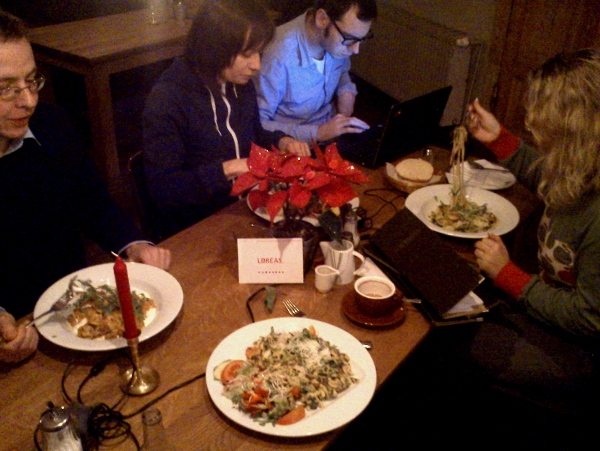
\includegraphics{editorial.jpg}
\caption{Redaktionsorte VIII (Berlin-Friedrichshain, Dezember 2014)}
\end{figure}

Weitere Beiträge beschäftigen sich mit dem Konzept einer
informationellen Stadt mit ubiquitären Diensten und stellt anhand der
Ergebnisse einer Befragung beispielhaft die Situation der
südkoreanischen Stadt New Songdo City dar, erläutert von der Gewinnerin
des SWIF 2014 Aylin Ilhan. Andreas Degkwitz spricht sich für eine
Entwicklung der Zentralbibliothek von einer Special Subject Collections
hin zu einem Discipline Driven Information Provisioning aus, ein auf dem
17th Fiesole Collection Development Retreat am 06.05.2015 in Berlin
gehaltenen Vortrag, den wir freundlicherweise veröffentlichen dürfen.

Rezensionen kommen diesmal von Übersee zu Information Services Today und
vom Über-den-Tellerrand, bei der wir über den Bibliotheksbezug in der
Pop-Rock-Musik erfahren. Eventuell wird dies zur künftigen Kolumne.

\begin{center}\rule{0.5\linewidth}{\linethickness}\end{center}

Im Sommer dieses Jahres wird \emph{LIBREAS.Library Ideas} zehn Jahre
alt, was eine auch für uns als Redaktion erstaunliche Zeitspanne ist.
Sind wir wirklich schon so alt geworden? Haben wir schon unseren
jugendlichen Elan hinter uns gelassen oder hatten wir nie welchen? Haben
wir unsere Träume aufgegeben? Haben wir uns zumindest inhaltlich
gefunden? (Haben wir noch nicht, immer noch sind wir über die
Zuschreibungen von aussen erstaunt, die unserer Projekt mal als
Studentenzeitschrift und mal als zu anspruchsvoll, mal als theoretisches
Organ und mal als Feuilleton, mal als akzeptierten Publikationsort und
mal als kritisches Organ im Bibliothekswesen bezeichnen.)

Und dennoch: Zehn Jahre sind eine lange Zeit, in der nicht nur die
Zeitschrift, sondern auch wir uns verändert und uns in verschiedene
Richtung gehen lassen haben. Deshalb trauen wir uns, einmal zu unserer
Grundfrage und Grundhaltung zurückzukehren und in einem Symposium die
Frage diskutieren zu lassen, was die \emph{Bibliothek als Idee}
eigentlich genau ist. Dieses Symposium gestalten wir aus dem Bauch
heraus, so wie wir uns ein interessantes Treffen, das wir besuchen
wollten, vorstellen (so wie wir eine Zeitschrift zu gestalten versuchen,
die wir lesen wollen würden) und das beinhaltet auch, unsere Leserinnen
und Leser --- und vor allem die Mitglieder des LIBREAS. Vereins --- für
das Spätsommer-Wochenende vom 12./13. September 2015 nach Berlin
einzuladen, zu Symposium, Diskussion, Feterei, gemeinsamen Frühstück wie
es Berliner mögen und Vereinssitzung, die jährlich stattfindet.
Referentinnen und Referenten, Ort und weitere Metadaten berichten wir
über unsere etablierten elektronischen Kanäle.

Eure / Ihre Redaktion LIBREAS. Library Ideas

(Berlin, Bielefeld, Chur, München, Potsdam)

%autor

\end{document}